\let\negmedspace\undefined
\let\negthickspace\undefined
\documentclass[journal]{IEEEtran}
\usepackage[a5paper, margin=10mm, onecolumn]{geometry}
\usepackage{tfrupee} 

\setlength{\headheight}{1cm}
\setlength{\headsep}{0mm}

\usepackage{gvv-book}
\usepackage{gvv}
\usepackage{cite}
\usepackage{amsmath,amssymb,amsfonts,amsthm}
\usepackage{algorithmic}
\usepackage{graphicx}
\usepackage{textcomp}
\usepackage{xcolor}
\usepackage{txfonts}
\usepackage{listings}
\usepackage{enumitem}
\usepackage{mathtools}
\usepackage{gensymb}
\usepackage{comment}
\usepackage[breaklinks=true]{hyperref}
\usepackage{tkz-euclide} 
\usepackage{listings}

\def\inputGnumericTable{}                                 
\usepackage[latin1]{inputenc}                                
\usepackage{color}                                            
\usepackage{array}                                            
\usepackage{longtable}                                       
\usepackage{calc}                                             
\usepackage{multirow}                                         
\usepackage{hhline}                                           
\usepackage{ifthen}                                           
\usepackage{lscape}

\title{\textbf{1.8.23}}
\author{\textbf{EE25BTECH11006 - ADUDOTLA SRIVIDYA}}
\date{september 13, 2025}

\begin{document}

\maketitle

Question:\\
 If the point $\textbf{A}(2,-4)$ is equidistant from $\textbf{P}(3,8)$ and $\textbf{Q}(-10,y)$, find the values of $y$.
 Also find distance $\vec{PQ}$.

\solution:\\
The input parameters for this problem are available in Table 
\begin{tabular}{|c|c|}
\hline
\textbf{Name} & \textbf{Value} \\ \hline
$\vec{A}$ & $\myvec{2 & 1 \\0 & 3}$ \\ \hline
\end{tabular}


Since $\vec{A}$ is equidistant from $\vec{P}$ and $\vec{Q}$,

\begin{align}
    \norm{\myvec{\vec{A} - \vec{P}}} = \norm{\myvec{\vec{A} - \vec{Q}}}
\end{align}

\begin{align}
     \norm{\myvec{\vec{A} - \vec{P}}}^2 = \norm{\myvec{\vec{A} - \vec{Q}}}^2
\end{align}

\begin{align}
    {(\vec{A} - \vec{P})}^\top (\vec{A} - \vec{P}) \, &= \, {(\vec{A} - \vec{Q})}^\top (\vec{A} - \vec{Q})
\end{align}

\begin{align}
 {||\vec{A}||}^2 \, - \, 2\vec{A}^\top\vec{P} \, + \, {||\vec{P}||}^2 \, = \, {||\vec{A}||}^2 \, - \, 2\vec{A}^\top\vec{Q} \, + \, {||\vec{Q}||}^2
\end{align}

\begin{align}
    {(\vec{P} - \vec{Q})}^\top \vec{A} \, &= \, \frac{{||\vec{P}||}^2\, - \, {||\vec{Q}||}^2}{2}
\end{align}


After substituting the values,

\begin{align}
    \myvec{3-(-10)\\8-y}^\top\myvec{2\\-4}\, = \, \frac{73-(-10)^2 -y^2}{2}
\end{align}

\begin{align}
    y^2 +8y + 15 = 0
\end{align}

Therefore,
\begin{align}
    y \, = -5 , -3
\end{align}

\begin{align}
   \vec{Q_1} = \myvec{-10 \\ -5}, \quad
   \vec{Q_2} = \myvec{-10 \\ -3}
\end{align}

\begin{align}
    \norm{\myvec{\vec{P} - \vec{Q_1}}} &= \left\|\myvec{3\\8} - \myvec{-10\\-5}\right\| \\
    &= \left\|\myvec{13\\13}\right\| \\
    &= 13\sqrt{2}
\end{align}

\begin{align}
    \norm{\myvec{\vec{P} - \vec{Q_2}}} &= \left\|\myvec{3\\8} - \myvec{-10\\-3}\right\| \\
    &= \left\|\myvec{13\\11}\right\| \\
    &= \sqrt{290}
\end{align}

\begin{figure}[H]
\centering
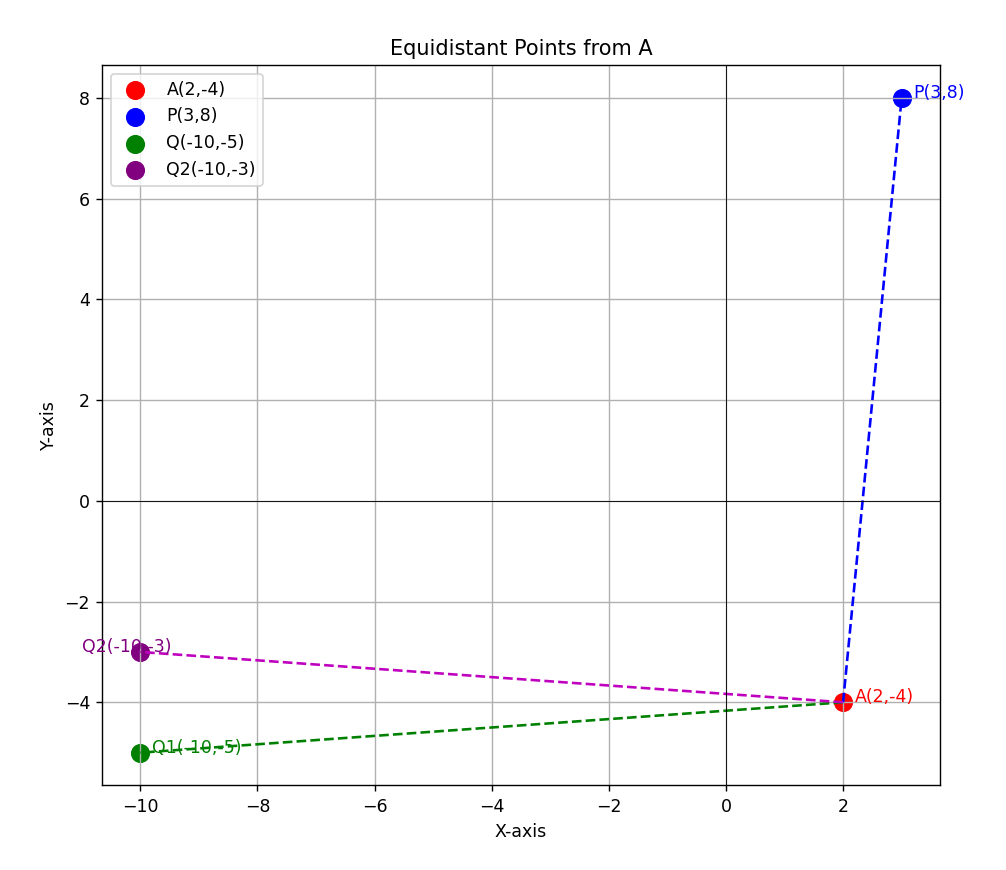
\includegraphics[width=0.56\columnwidth]{figs/fig1.png}
 \caption*{Equidistant Points from $\vec{A}$ with Distances}
\label{fig:graph.png}
\end{figure}


\end{document}